\documentclass{standalone}
\usepackage{ tikz }
\usepackage{ xparse }
\usepackage{ amsmath }
\usepackage{../../../macros}

\begin{document}
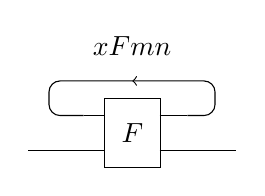
\begin{tikzpicture}[yscale=-1,x=1em,y=1.25em]

    \node at (3,-1.5) {$\morph{\trace{x}{F}}{m}{n}$};
    \draw (-0.75,1.5) -- (1.25,1.5);
    \draw (1.25,1.5) -- (2,1.5);
    \draw (4.0,0.5) -- (5.0, 0.5);
    \draw [rounded corners, ->] (5.0,0.5) -- (6.0,0.5) -- (6.0,-0.5) -- (3,-0.5);
    \draw [rounded corners] (3,-0.5) -- (0,-0.5) -- (0,0.5) -- (1.25,0.5);
    \draw (1.25,0.5) -- (2,0.5);
    \draw (4.0,1.5) -- (5.25,1.5);
    \draw (5.25, 1.5) -- (6.75, 1.5);

    \node[draw, minimum height = 2.5em, minimum width = 2em, anchor = west] at (2,1){$F$};
\end{tikzpicture}
\end{document}